\chapter{Cloud-Edge}

\section{Cloud Computing}
Il \textbf{Cloud Computing} è un insieme di tecnologie che permettono di compiere operazioni
di elaborazione, networking e archiviazione di dati utilizzando risorse hardware/software distribuite (tipicamente remote) e virtualizzate. Le principali caratteristiche che contraddistinguono questa tecnologia sono:
\begin{itemize}
	\item \textbf{On-demand self-service}: Un customer può unilateralmente rifornirsi di
	capacità di calcolo senza interazione umana.
	\item \textbf{Broad network access}: Le risorse sono disponibili in rete e sono accessibili
	tramite meccanismi standard.
	\item \textbf{Resource pooling}: Le risorse fornite dal provider sono distribuite
	dinamicamente a più utenti, realizzando un modello multi-tenant.
	\item \textbf{Rapid elasticity}: e risorse possono essere fornite e rilasciate in modo elastico, e in alcuni casi automatico, così da scalare rapidamente in accordo con la
	richiesta.
	\item \textbf{Measured service}: Il sistema cloud controlla ed ottimizza l'uso delle risorse,
	monitorandolo.
\end{itemize}
Nel modello classico di gestione dei servizi IT (on-premise), un’azienda acquisisce e
gestisce in-house le soluzioni hardware e software necessarie al proprio business. Questo significa che l’azienda è proprietaria dell’hardware e delle licenze del software che utilizza, e che il personale IT (interno/esterno all’azienda) si occupa della loro completa gestione. Nel modello Cloud invece, le risorse sono ospitate all’interno dell’infrastruttura di
proprietà del provider, e le aziende possono accedervi in qualsiasi momento attraverso
piattaforme applicative accessibili via web. I servizi Cloud possono essere erogati secondo diversi modelli di servizio e di fornitura, in modo che un’azienda possa scegliere in base alle proprie esigenze.

\subsection{Architettura di un servizio Cloud}
L'\textbf{architettura di un generico servizio Cloud} viene definita dal NIST attraverso la figura che segue [\ref{fig:nist-model}], definisce cosa ciascun servizio deve fare e non come debba essere implementato.
\begin{figure}[!h]
	\centering
	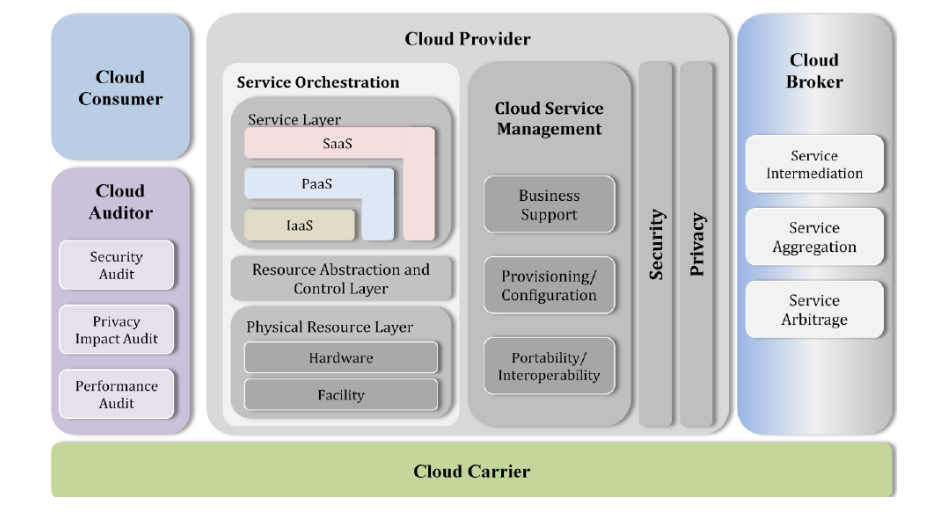
\includegraphics[width=0.55\linewidth]{img/nist-model.png}
	\caption{Modello NIST per il Cloud Computing.}
	\label{fig:nist-model}
\end{figure}
Si individuano 5 \textit{attori} principali, ossia entità (sistema o persona) che partecipa ad una transazione o processo del sistema Cloud.
\begin{itemize}
	\item \textbf{Cloud consumer}: Utilizza servizi offerti da Cloud
	providers.
	\item \textbf{Cloud provier}: \MakeUppercase{è} responsabile di rendere servizi
	disponibili a parti interessate.
	\item \textbf{Cloud auditor}: Conduce una valutazione indipendente
	dei servizi cloud, delle operazioni del sistema
	informativo, delle prestazioni e della sicurezza del
	sistema Cloud.
	\item \textbf{Cloud broker}: Gestisce l'uso, le performance e la
	distribuzione dei servizi cloud; negozia le relazioni tra
	provider e consumer.
	\item \textbf{Cloud carrier}: Intermediario che fornisce connettività e
	trasporto dei servizi cloud, da provider e consumer.
\end{itemize}

\subsection{Modelli di servizio}
I \textbf{modelli di servizio} riguardano che tipo di risorsa IT il provider fornisce. Le tre tipologie principali sono le seguenti.
\begin{itemize}
	\item \textbf{SaaS (Software-as-a-service)}: Acquisizione di intere
	applicazioni software in esecuzione su infrastrutture Cloud e accessibili da remoto on-demand. In questo caso è il provider a gestire l’aggiornamento, la manutenzione, la
	scalabilità e le responsabilità in termini di sicurezza. Dunque, il customer non deve affrontare spese riguardanti queste gestioni. Si specifica che il software è di possesso del provider, il customer paga quindi per poter mantenere il servizio attivo e raggiungibile da altri utenti.
	\item \textbf{IaaS (Infrastructure-as-a-service)}: Acquisizione di una
	infrastruttura virtuale al di sopra delle quali il customer può installare ed eseguire software arbitrario. L’utente non può gestire l’infrastruttura sottostante, ma ha il
	controllo su sistema operativo, storage, applicazioni e un controllo limitato
	su alcuni componenti di rete, come i firewall. Quelle che sono messe a disposizione sono quindi sono features hardware, per tale motivo all’IaaS ci si riferisce spesso come
	HaaS (Hardware as a Service).
	\item \textbf{PaaS (Platform-as-a-service)}: Acquisizione di ambienti e
	tool web-based per lo sviluppo, il testing, la messa in
	esercizio, l’hosting e la manutenzione delle proprie
	applicazioni.
\end{itemize}

\subsection{Modelli di fornitura}
I \textbf{modelli di fornitura} riguardano dove e da chi è ospitato il Cloud. Si individuano tre tipologie principali.
\begin{itemize}
	\item \textbf{Cloud pubblico}: Il servizio è fornito da un provider terzo (es. AWS), quindi le risorse sono condivise tra più clienti (multi-tenant). La scalabilità è alta e i costi sono contenuti, ma c'è meno controllo diretto.
	\item \textbf{Cloud privato}: Il servizio è dedicato a un’unica organizzazione, quindi può essere gestito internamente o da un provider esterno. C'è più controllo e sicurezza, ma i costi di gestione sono più alti.
	\item \textbf{Cloud ibrido}: \MakeUppercase{è} una combinazione di pubblico e privato. Le risorse possono muoversi tra i due, ad esempio si tengono dati sensibili nel cloud privato e quelli meno critici nel pubblico.
\end{itemize}

\subsection{Rischi e Sicurezza}
In generale, affidandosi al Cloud si perde (totalmente o parzialmente, a
seconda del modello di servizio e di fornitura scelto) il controllo dei propri dati
e sistemi, e ci si espone a dei \textbf{rischi di sicurezza} che dipendono sia dalle misure
di sicurezza implementate dall’utente nelle proprie applicazioni che dalle
politiche di protezione implementate dal fornitore del servizio Cloud (modello
di responsabilità condivisa). Oltre ai classici requisiti di sicurezza, esistono poi dei vincoli minimi in termini di sicurezza ed affidabilità richiesti dalle norme vigenti nazionali ed europee, che non tutti i servizi Cloud disponibili potrebbero essere in grado di rispettare.
\\
\\
ENISA (European Network and Information Security Agency) riporta i principali rischi di sicurezza del Cloud, i quali andrebbero tenuti d'occhio e cercati di mitigare per quanto possibile. 

\section{IoT}
\textbf{Internet of Things} (IoT) viene generalmente definito come:
\\
\\
\textit{"Un’infrastruttura globale per la società dell’informazione, che abilita servizi avanzati interconnettendo cose (fisiche e virtuali) basate su informazioni e comunicazioni interoperabili, esistenti e in evoluzione tecnologie"}. 
\\
\\ 
I dispositivi coinvolti in un Sistema IoT possono essere anche molto eterogenei in quanto a capacità di elaborazione e memorizzazione, connettività e alimentazione. Alcuni tra i campi di applicazione sono: smart factory, smart home, smart city, e-Health (monitoraggio dei pazienti a distanza) e smart energy.

\subsection{Architettura di un sistema IoT}
Un sistema IoT si sviluppa solitamente tramite un'\textbf{architettura a 3 livelli}:
\begin{itemize}
	\item \textbf{Livello dei dispositivi}: Comprende sensori, attuatori, e sistemi embedded in grado di generare tipicamente grosse moli di dati.
	\item \textbf{Livello di connettività}: Include i protocolli che consentono ai dispositivi di comunicare con il livello dei servizi e applicazioni.
	\item \textbf{Livello dei servizi e applicazioni}: Solitamente include servizi Cloud
	che si occupano di elaborare i dati generati dai dispositivi.
\end{itemize}

\subsection{Sicurezza}
I dispositivi IoT sono \textbf{insicuri per natura}: sono connessi e quindi potenzialmente accessibili e spesso non possiedono la capacità computazionale necessaria per proteggersi adeguatamente (ad esempio, attraverso la cifratura dei dati scambiati o l’utilizzo di meccanismi di autenticazione). 
\\
\\
Data la grandissima diffusione di dispositivi IoT in svariati contesti, essi sono
particolarmente soggetti ad attacchi di tipo ransomware, denial of service, furto di identità
e di dati, man-in-the-middle e altri, che possono avere effetti estremamente negativi non
solo in termini di security in sè (confidenzialità, integrità e disponibilità), ma anche sulla
privacy e sulla safety.
\\
\\
Per garantire adeguata protezione, è necessario prevedere meccanismi di sicurezza che si
adattino alle capacità dei singoli dispositivi (ad esempio, meccanismi di cifratura
lightweight basati su architetture hardware a basso impatto) e che siano in grado di
assicurare, fra gli altri, autenticazione, controllo degli accessi e sicurezza dei canali di
comunicazione.

\section{Edge Computing}
Il termine \textbf{Edge Computing} significa letteralmente \textit{"elaborazione ai margini"}, ovvero elaborazione delle informazioni in prossimità della relativa sorgente. L’Edge Computing nasce per rispondere all’esigenza di ridurre la latenza e il consumo di banda che caratterizzano tipicamente i sistemi IoT classici, in cui grossi moli di dati vengono inviati ai servizi Cloud per elaborazioni successive. Il paradigma Edge, inoltre, consente di ridurre i rischi di sicurezza legati alla delocalizzazione dei dati, che potrebbero avere in taluni casi requisiti stringenti di sicurezza/privacy.

\subsection{Architettura}
I componenti principali nell'\textbf{architettura di un sistema di Edge Computing} sono:
\begin{itemize}
	\item \textbf{Edge devices}: Dispositivi edge e IoT attrezzati per
	raccogliere dati ed eseguire elaborazioni in locale.
	\item \textbf{Edge server o gateway}: Server perimetrali utilizzati per distribuire le applicazioni sui dispositivi. Sono in costante comunicazione con i dispositivi
	utilizzando degli agenti installati su ciascuno di questi.
	\item \textbf{Edge network o micro data center}: Tecnologie
	di rete avanzate. Possono essere immaginate come un cloud locale con cui i dispositivi possono comunicare.
	\item \textbf{Enterprise Hybrid Cloud}:	Si occupa
	dell'archiviazione e la gestione dei dati a livello aziendale (analisi complesse e dashboard).
\end{itemize}

\begin{figure}[!h]
	\centering
	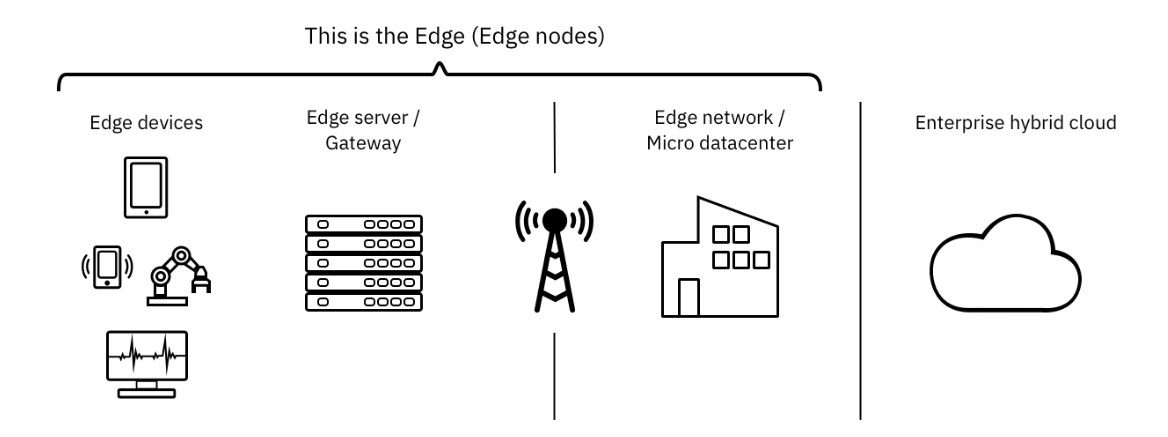
\includegraphics[width=0.55\linewidth]{img/edge.png}
	\caption{Architettura di un sistema di Edge Computing.}
	\label{fig:edge}
\end{figure}

\section{Fog Computing (cenni)}
Per \textbf{Fog Computing} si intende un paradigma per l’elaborazione dati che calca alcuni dei
principi del paradigma di Cloud Computing, rispondendo tuttavia ad alcune limitazioni che
quest’ultimo presenta. Nonostante non esiste una definizione univoca per questo paradigma, analizzando le diverse definizione attribuite è possibile osservare una serie di punti in comune che ne definiscono le proprietà principali:
\begin{itemize}
	\item \textbf{Decentralizzazione dei servizi}: Offre dei servizi dislocati su nodi
	fisicamente disaccoppiati e geograficamente distribuiti.
	\item \textbf{Architettura gerarchica}:	L'organizzazione avviene per livelli, ciascuno dei quali ha un ruolo specifico (raccogliere, elaborare e inoltrare i dati).
\end{itemize}
Per quanto detto le similitudini con il classico Edge Computing sono molte, motivo per cui i due sono spesso confusi, tuttavia sono due le cose che contraddistinguono il Fog Computing:
\begin{itemize}
	\item In generale, i Fog Node sono tipicamente schierati nelle
	posizioni intermedie fra i nodi Edge e i servizi Cloud.
	\item A differenza degli Edge Node, le capacità di calcolo, immagazzinamento dati e
	networking dei Fog Node sono nettamente superiori.
\end{itemize}

\section{Virtualizzazione}
La \textbf{virtualizzazione} è una tecnologia che consente di creare una versione virtuale (cioè simulata via software) di qualcosa che normalmente è fisico o reale, come un sistema operativo o un computer.
\\
\\
Che sia eseguita in hardware, software o incorporata in sottosistemi, la virtualizzazione viene
sempre ottenuta utilizzando e combinando tre semplici tecniche [\ref{fig:virtualiz}]. 
\begin{figure}[!h]
    \centering
    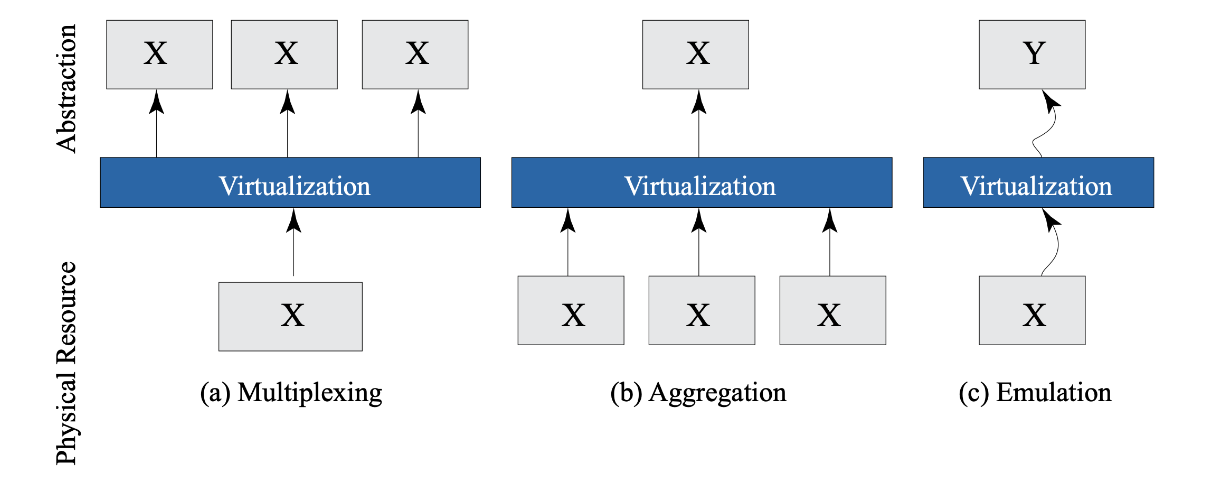
\includegraphics[width=0.6\linewidth]{img/virtualizzazione.png}
    \caption{Le tre tecniche base di virtualizzazione.}
    \label{fig:virtualiz}
\end{figure}
\begin{itemize}
	\item Il \textbf{multiplexing} espone una risorsa tra più entità virtuali. Ce ne sono due
	tipologie, nello spazio e nel tempo. Con il multiplexing \textit{nello spazio}, la risorsa
	fisica viene partizionata in entità virtuali. Ad esempio, il sistema operativo
	multiplexa diverse pagine di memoria fisica su diversi spazi di indirizzi. Con il multiplexing \textit{temporale}, la stessa risorsa fisica viene programmata temporalmente tra entità virtuali. Ad esempio, lo scheduler del sistema operativo suddivide i core della CPU tra l’insieme di processi eseguibili.
	\item L’\textbf{aggregazione} fa il contrario, raggruppa più risorse fisiche e le fa apparire come un'unica entità. Ad esempio, un controller RAID aggrega più dischi in un unico
	volume. Una volta configurata, l'interfaccia delle risorse fisiche deve apparire come unica, per cui l'utilizzatore è del tutto ignaro del processo di aggregazione.
	\item Infine, con l'\textbf{emulazione}, invece di accedere direttamente all'hardware reale, il programma accede a un "livello software" che finge di essere un certo hardware. L'emulatore crea un finto dispositivo che si comporta come uno vero, anche se quel dispositivo non esiste fisicamente nel computer. Ad esempio, gli emulatori tra architetture eseguono un’architettura del processore su un’altra.
\end{itemize}
Le tre tecniche possono essere combinate per formare uno stack di esecuzione completo.

\subsection{Macchine virtuali}
Una \textbf{macchina virtuale} è un ambiente di elaborazione completo con capacità di elaborazione, memoria e canali di comunicazione isolati. \MakeUppercase{è} possibile fare la seguente classificazione.
\begin{itemize}
    \item \textbf{Macchine virtuali basate sul linguaggio}, come \textit{Java Virtual Machine}.
    \item \textbf{Macchine virtuali leggere}, che si basano su una combinazione di meccanismi di
    isolamento hardware e software per garantire che le applicazioni in esecuzione direttamente sul processore siano isolate in modo sicuro da altre e dal sistema operativo sottostante. Un esempio sono i \textit{container}.
    \item \textbf{Macchine virtuali a livello di sistema}, in cui viene emulato l'intero hardware di un calcolatore, permettendo di installare un sistema operativo intero. Le piattaforme che permettono di eseguire questa tipologia di macchine virtuali sono:
    \begin{itemize}
        \item \textit{Hypervisor}: Si basa sull'esecuzione diretta sulla CPU per la massima efficienza.
        \item \textit{Simulatore di macchina}: Implementato come una normale applicazione a livello utente.
    \end{itemize}
\end{itemize}

\subsection{Hypervisor}
Un \textbf{hypervisor} (o Virtual Machine Monitor - VMM) è un software di sistema che permette di creare ed eseguire macchine virtuali, con l'obiettivo di ridurre al minimo i costi di esecuzione. Quando più VM coesistono simultaneamente sullo stesso sistema di computer, l’hypervisor multiplexa (cioè alloca e
schedula) le risorse fisiche in modo appropriato tra le macchine virtuali. Le architetture dell’hypervisor possono essere classificate come segue [\ref{fig:hyper-type}].
\begin{itemize}
    \item \textbf{Tipo 1 (bare-metal)}: Il VMM viene eseguito direttamente sull'hardware macchina host (bare), senza necessità di un sistema operativo.
    \item \textbf{Tipo 2 (hosted)}: Il VMM viene eseguito su un host esteso, sotto il sistema operativo host.
\end{itemize}
\begin{figure}[!h]
    \centering
    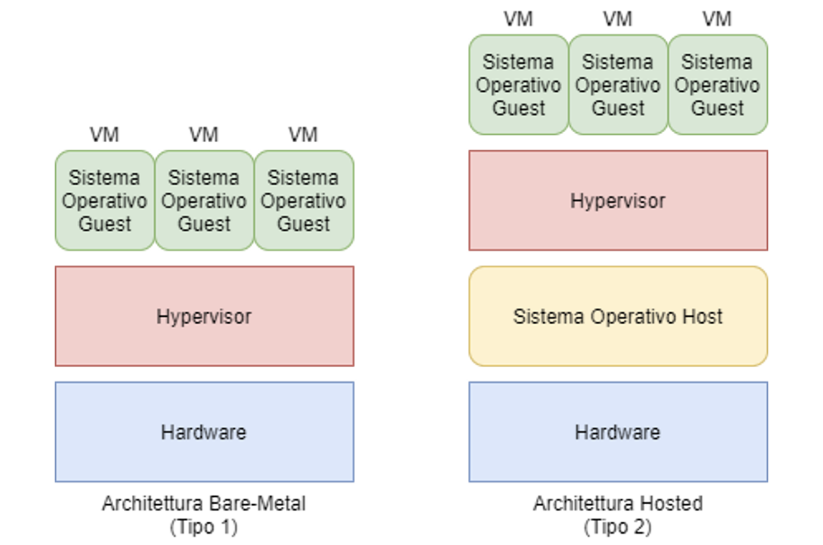
\includegraphics[width=0.6\linewidth]{img/hyperv-types.png}
    \caption{Tipologie di hypervisor.}
    \label{fig:hyper-type}
\end{figure}
In entrambi i tipi, il VMM crea la macchina virtuale. Tuttavia, in un ambiente di tipo 1, il
VMM sulla macchina bare deve eseguire anche lo scheduling del sistema e l'allocazione (reale)
delle risorse. Di conseguenza, il VMM di tipo 1 può dover includere tale codice, non specificamente
necessario per la virtualizzazione. In un sistema di tipo 2, le funzioni di allocazione delle
risorse e creazione dell'ambiente per la macchina virtuale sono eseguiti dal sistema operativo host.
\\
\\
Osserviamo come l'enfasi sulla differenza tra i due sia sull'allocazione delle risorse e non sul fatto che l’hypervisor venga eseguito in modalità privilegiata o meno. In particolare, un hypervisor può essere di tipo 2 anche quando viene eseguito in modalità kernel, ad esempio \textit{VMware Workstation} funziona in questo modo.
\\
\\
Nella sua forma più elementare, un hypervisor utilizza due delle tre tecniche di virtualizzazione: multiplexa (nello spazio e possibilmente nel tempo) il processore fisico ed emula tutto il resto, in particolare i dispositivi I/O. Questa combinazione di tecniche è necessaria e sufficiente nella pratica per raggiungere i criteri
di efficienza. Il motivo è che se non si multiplexa bene la CPU e la MMU (Memory Management Unit), l’hypervisor sarebbe costretto a simulare tutto, rendendo le VM molto lente.
\\
\\
In modo molto simile a come la scheduler gestisce l'esecuzione di diversi processi sullo stesso processore, anche l’hypervisor deve decidere quale VM può utilizzare la macchina. Dunque, l'hypervisor carica nel processore i registri della VM attiva, le sue tabelle di memoria e la lascia eseguire. Ovviamente, l’hypervisor è anche responsabile di garantire la proprietà di sicurezza
della macchina virtuale. Assicura quindi che la CPU virtuale venga sempre eseguita con
privilegi ridotti, ad esempio non facendogli eseguire istruzioni privilegiate.
\\
\\
Per comprendere come avvenga la \textbf{gestione delle istruzioni privilegiate}, è necessario inanzitutto distinguere:
\begin{itemize}
    \item \textbf{Dynamic Binary Translation (DBT)}: L'intero codice della macchina virtuale viene eseguito normalmente, ma se viene richiamata qualche istruzione privilegiata, l'hypervisor la intercetta e tenta di tradurla in una equivalente e sicura. L'istruzione tradotta viene eseguita sul vero processore. Inoltre, questa viene salvata in una cache, così che il processore possa eseguirla nuovamente in futuro senza ritradurla.
    \item \textbf{Full-virtualization}: La macchina virtuale crede di essere su un vero computer fisico, e non sa di essere "virtuale". In questo caso l’hypervisor emula tutto l'hardware e il sistema operativo guest non deve essere modificato. Se prova ad eseguire istruzioni privilegiate, scatta una \textit{trap} e l’hypervisor interviene (trap-and-emulate). Il vantaggio è la possibilità di installare qualsiasi sistema operativo senza modificarlo, mentre lo svantaggio è l'overhead dovuto all'intercettazione delle istruzioni privilegiate.
    \item \textbf{Para-virtualization}: Il sistema operativo sa che sta girando in una macchina virtuale e collabora con l’hypervisor. In questo caso, il sistema operativo guest viene modificato per chiamare direttamente l’hypervisor quando deve fare operazioni privilegiate, per cui non si usano trap, ma chiamate specifiche dette \textit{hypercalls}. Il vantaggio è la rapidità, mentre lo svantaggio è l'uso di soli i sistemi operativi modificati per supportare questo tipo di virtualizzazione.
\end{itemize}
Osserviamo con qualche dettaglio in più il processo della \textit{trap and emulate}.
\begin{enumerate}
    \item Il sistema operativo guest esegue codice normalmente sul processore reale.
    \item Il processore incontra un'istruzione privilegiata, come un cambio di modalità di esecuzione (da utente a root).
    \item Il processore blocca l’istruzione e genera una \textit{trap}. Il controllo passa quindi al supervisore (che gira a un livello più alto, o con più privilegi, del guest).
    \item L’hypervisor simula via software il comportamento dell’istruzione.
    \item Dopo l’emulazione, l’esecuzione torna al sistema operativo guest.
\end{enumerate}

\begin{figure}[!h]
    \centering
    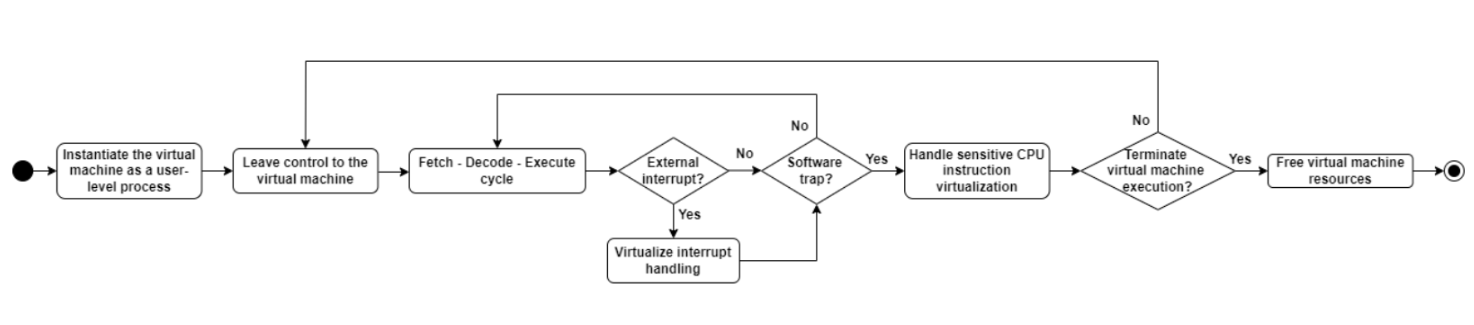
\includegraphics[width=1.1\linewidth]{img/trap-and-emulate.png}
    \caption{Flusso della tecnica trap and emulate.}
    \label{fig:trap-and-emulate}
\end{figure}

\subsection{Architetture Intel x86-64}
Le CPU Intel definiscono 4 \textbf{privilegi di esecuzione}, anche detti \textit{ring} [\ref{fig:rings}]. Il primo livello (ring 0) è il privilegio più alto, mentre il quarto (ring 3) è il più basso. Ciascuna istruzione deve essere gestita secondo privilegi di esecuzione adeguati. Ad esempio, il codice utente viene eseguito sul ring 3, mentre le funzioni del kernel (come ISR o system calls) devono essere eseguite su ring più bassi. In generale, l'esecuzione di istruzioni su ring non adatti porta alla generazione di trap o effetti inattesi.
\begin{figure}[!h]
    \centering
    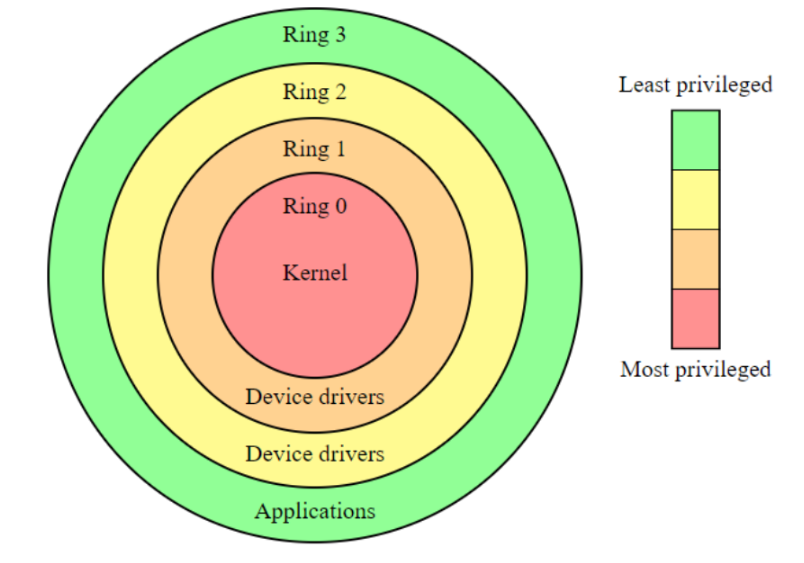
\includegraphics[width=0.5\linewidth]{img/rings.png}
    \caption{Privilegi di esecuzione nelle CPU Intel.}
    \label{fig:rings}
\end{figure}
Nelle CPU Intel, gli eventuali sistemi operativi guest eseguono nei ring 1-3. In caso di invocazione di istruzioni privilegiate, il controllo viene passato all'hypervisor, che esegue nel ring 0 e le gestisce con una tecnica di emulazione del tipo DBT [\ref{fig:intel-guestos}].
\begin{figure}[!h]
	\centering
	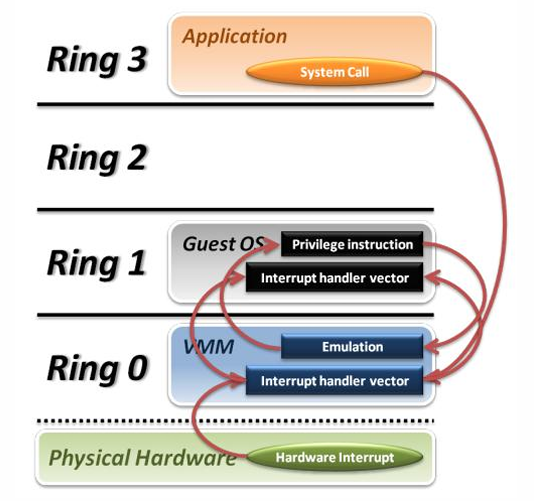
\includegraphics[width=0.45\linewidth]{img/intel-guestos}
	\caption{Gestione delle istruzioni privilegiate del guest os in Intel.}
	\label{fig:intel-guestos}
\end{figure}
Spostiamo ora la nostra attenzione sulle \textbf{architetture Intel x86-64} e cerchiamo di capire se su queste sia possibile adottare una tecnica del tipo \textit{trap and emulate}. Innanzitutto, le CPU Intel x86-64 posseggono un ISA di istruzioni privilegiate che non sono in grado di generare traps via software quando eseguite nel livello utente (ring 1-3). Per tale motivo, teoricamente queste architetture non si dimostrano adatte per il meccanismo di trap and emulate. Per risolvere questa limitazione, sono stati introdotti vari supporti:
\begin{enumerate}
    \item Estensione dell'ISA.
    \item Registri che implementano strutture di controllo per gestire le macchine virtuali.
    \item Meccanismi hardware per aggiornare i registri con le informazioni principali del cambio di contesto tra macchina virtuale e hypervisor.
\end{enumerate}
\textbf{Intel VT-x} è l'estensione hardware che permette il supporto della virtualizzazione nelle architetture x86-64. Questa aggiunge al processore due modalità di esecuzione speciali, ciascuna delle quali ha sempre i classici 4 livelli di privilegio (rings).
\begin{itemize}
    \item \textbf{VMX Root Operation}: Modalità in cui gira l’hypervisor (cioè il software che controlla le VM), ha il pieno controllo dell’hardware.
    \item \textbf{VMX Non-Root Operation}: Modalità in cui girano le macchine virtuali guest, sembrano avere il controllo dell’hardware ma in realtà sono sorvegliate dall’hypervisor.
\end{itemize}
Il cambio di modalità operativa avviene in automatico se la VM in modalità non-root tenta di eseguire un'istruzione privilegiata (il cambio potrebbe non avvenire se il sistema non è configurato per farlo). L'hardware mantiene due tipi di informazioni di stato (registri, flag, eccetera), la \textit{guest-area} (per le macchine virtuali) e la \textit{host-area} (per il sistema host). In particolare, la \textbf{Virtual Machine Control Structure} (VMCS) è una struttura speciale gestita dal processore che contiene tutte le informazioni necessarie per gestire il passaggio tra le due modalità e salvare/ripristinare lo stato del processore quando avviene il cambio di contesto. Il cambio di contesto tra macchina virtuale e macchina host (e viceversa) avviene mediante:
\begin{itemize}
    \item \textbf{VM Entry}: Il processore passa dal sistema host alla macchina virtuale guest, per cui viene ripristinato lo stato presente nella guest-area.
    \item \textbf{VM Exit}: La VM cerca di eseguire un'istruzione che richiede l’intervento dell’hypervisor.
\end{itemize}
Con una tale gestione della virtualizzazione, il flusso di esecuzione delle macchine virtuali può procedere normalmente: non è richiesta alcuna re-implementazione delle primitive del guest-os. In caso di istruzioni privilegiate, viene avviata una VM Exit che permette di procedere emulando l'istruzione [\ref{fig:vm_flusso}].
\begin{figure}[!h]
	\centering
	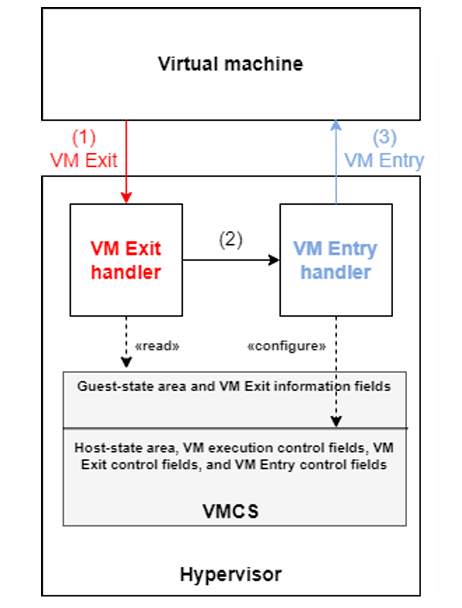
\includegraphics[width=0.45\linewidth]{img/vm-flusso}
	\caption{Flusso di esecuzione per istruzioni privilegiate della VM.}
	\label{fig:vm-flusso}
\end{figure}
Le istruzioni eseguite in modalità VMX Non-Root che causano una VM Exit sono:
\begin{itemize}
	\item \textit{Istruzioni che causano VM Exit incondizionatamente}, ovvero istruzioni che fanno sempre scattare un VM Exit, indipendentemente dalla configurazione del sistema. Un esempio è \textit{CPUID} che restituisce informazioni sul processore.
	\item \textit{Istruzioni che causano VM Exit condizionatamente}, ovvero istruzioni possono causare un VM Exit, ma solo se configurato così nel controllo VMCS. L'hypervisor specifica quindi quali istruzioni rientrano in questa categoria.
	\item \textit{Eccezioni}, quando il guest genera un’eccezione.
	\item \textit{Interrupt esterni}, dovuti a periferiche.
	\item \textit{Non-Maskable Interrupts} (NMIs), tipicamente usate per condizioni critiche come errori hardware.
\end{itemize}
Anche nel caso di interruzioni esterne, il comportamento del sistema è molto simile. Queste infatti generano un VM Exit appositamente gestito dall'hypervisor, il quale:
\begin{itemize}
    \item Se la macchina virtuale ha le interruzioni disabilitate, l'hypervisor avvia una VM Entry specificando che la VM Exit accadrà solo quando le interruzioni saranno abilitate.
    \item Se la macchina virtuale ha le interruzioni abilitate, l'hypervisor avvia una VM Entry trasferendo la richiesta di interruzione alla VM.
\end{itemize}
L'architettura Intel x86-64 supporta anche la \textbf{virtualizzazione della memoria} attraverso le due tecniche di indirizzamento lineare e paginazione. Con indirizzamento lineare si intende il processo di mappare gli indirizzi generati dalla CPU in uno spazio degli indirizzi virtuali per la memoria virtuale. Mentre la paginazione è ciò che consente di associare a ciascun indirizzo lineare al corrispondente indirizzo fisico [\ref{fig:virtual-mem}].
\begin{figure}[!h]
	\centering
	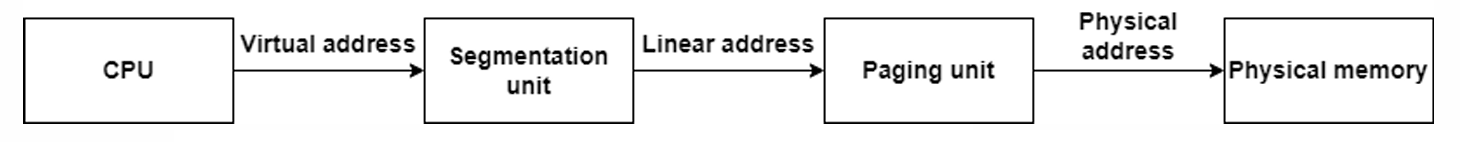
\includegraphics[width=0.8\linewidth]{img/virtual-mem}
	\caption{Processo di traduzione indirizzi da VM a sistema host.}
	\label{fig:virtual-mem}
\end{figure}
Gli indirizzi fisici generati dalle macchine virtuali vengono tradotti in indirizzi fisici per la macchina host tramite un meccanismo noto come \textit{Extended Page Table} (EPT), che fa tutto in hardware.